\documentclass[12pt,a4paper]{article}
\usepackage[utf8x]{inputenc}
\usepackage[portuges]{babel}
\usepackage{amsmath}
\usepackage{amsfonts}
\usepackage{amssymb}
\usepackage{graphicx}
\bibliographystyle{osa}
\usepackage[top=2cm, bottom=2cm, left=2cm, right=2cm]{geometry}

\author{Guilherme Bertoldo}
\title{Procedimento para gerar a tubeira otimizada de Rao}
\begin{document}
	\maketitle

\begin{itemize}
	\item Revisão 4 (15/05/2020): Na Eq.~19 do artigo do Rao falta um sinal negativo no lado esquerdo da igualdade.
	\item Revisão 3 (15/05/2020): Atualização no procedimento e nomenclatura das variáveis.
	\item Revisão 2 (07/05/2020): Correção do coeficiente de empuxo (na dedução foi definido como $E/(2A_t p_0)$ ao invés de $E/(A_t p_0)$). 
	\item Revisão 1 (24/04/2020): Erros de dedução e de digitação corrigidos.
	\item Revisão 0 (23/04/2020): Primeira versão do texto.
\end{itemize}

	Com base na Fig.~\ref{fig:nozzle}, onde $x$ e $y$ estão parametrizados em termos do raio da garganta, e considerando prescritos a distribuição do número de Mach, o ângulo $\theta$ do vetor velocidade com relação ao eixo $x$ ao longo da linha TT', bem como a razão $p_a/p_0$ (pressão ambiente/pressão de estagnação) e o número de Mach $M_E$ no ponto E, o procedimento para gerar a tubeira otimizada de Rao consiste nos seguintes passos: 
\begin{figure}[!ht]
\centering
\includegraphics[width=0.8\textwidth]{./fig/nozzle}
\caption{Esquema para a construção da tubeira de Rao (fonte: Rao, 1958)}
\label{fig:nozzle}
\end{figure}
\begin{enumerate}
	\item Gera-se características à direita a partir da seção de expansão TB'; 
	\item Determina-se o ângulo $\theta_E$ do vetor velocidade, e consequentemente da inclinação da parede, no ponto E com a Eq.~(14) do artigo de Rao. Em termos dos parâmetros adimensionais, esta equação é dada por
	\begin{equation}\label{eq:thetaE}
	\sin{(2\theta_E)}=\frac{2}{\gamma}\left(1-\frac{p_a}{p_0p_r(M_E)}\right)\frac{\sqrt{M_E^2-1}}{M_E^2},
	\end{equation}
	onde $\gamma$ é a razão de calores específicos e $p_r(M)$ é a razão entre a pressão local $p$ e a pressão de estagnação $p_0$:
	\begin{equation}\label{eq:pr}
	p_r(M)=\frac{p}{p_0}=\left(1+\frac{\gamma-1}{2}M^2\right)^{-\frac{\gamma}{\gamma-1}}.
	\end{equation}
	Obs.: No artigo de Rao, a Eq.~(\ref{eq:thetaE}) está escrita em termos de $\cot{\alpha}$, onde $\alpha$ é o ângulo de Mach. Considerando que 
	\begin{equation}\label{eq:sin_alpha}
	\sin{\alpha}=1/M
	\end{equation} 
	e
	\begin{equation}\label{eq:trig}
	\sin^2{\alpha}+\cos^2{\alpha}=1,
	\end{equation}
	então
	\begin{equation}\label{eq:cos_alpha}
	\cos{\alpha}=\frac{\sqrt{M^2-1}}{M},
	\end{equation} 
	\begin{equation}\label{eq:tan_alpha}
	\tan{\alpha}=\frac{1}{\sqrt{M^2-1}}
	\end{equation}
	e 
	\begin{equation}\label{eq:cot_alpha}
	\cot{\alpha}=\sqrt{M^2-1},
	\end{equation} 
	todos positivos, pois $0 < \alpha < 90^\circ$.
	\item As características à direita que emanam de TB' interceptam a superfície de controle (linha tracejada na Fig.~\ref{fig:control_surface} e linha CE na Fig.~\ref{fig:nozzle}). Este passo consiste primeiramente em determinar as coordenadas $(x_D,y_D)$ do ponto D e as coordenadas $(x_E,y_E)$ do ponto E da superfície de controle e, por fim, toda a linha DE. O procedimento é iterativo:
	\begin{figure}[!ht]
		\centering
		\includegraphics[width=0.8\textwidth]{./fig/control_surface}
		\caption{Determinação dos pontos B e D (fonte: Rao, 1958)}
		\label{fig:control_surface}
	\end{figure}
	
	\begin{enumerate}
		\item Escolhe-se uma característica à direita da seção TB', e.g. de $B_1$ a $D_1$. Determinam-se as coordenadas $(x_{D_1},y_{D_1})$ para as quais a Eq.~(17) do artigo de Rao é satisfeita:
		\begin{equation}\label{eq:Rao17}
		M^*\frac{\cos(\theta-\alpha)}{\cos{\alpha}}=M_E^*\frac{\cos(\theta_E-\alpha_E)}{\cos{\alpha_E}}
		\end{equation}
		onde 
		\begin{equation}\label{eq:M*}
		M^*=\left[\frac{1}{\gamma-1+\frac{2}{M^2}}\right]^{1/2}.
		\end{equation}
		Na Eq.~(\ref{eq:Rao17}) existe um intervalo de $M$ para o qual há dois valores de $\theta$. Por isso, numericamente, é conveniente determinar $M(\theta)$.
		\item Com as coordenadas $(x_{D_1},y_{D_1})$, determina-se $y_E$ através da Eq.~(18) do artigo de Rao:
		\begin{equation}\label{eq:Rao18}
		\eta=\frac{y}{y_E}=\frac{g(M_E,\theta_E)}{g(M,\theta)},
		\end{equation}
		onde
		\begin{equation}\label{eq:g}
		g(M,\theta)=\frac{M^2}{\sqrt{M^2-1}}p_r(M)\sin^2{\theta}.
		\end{equation}
		\item Com os valores de $(x_{D_1},y_{D_1})$ e $y_E$, avalia-se se a Eq.~(19) do artigo de Rao é satisfeita (o sinal negativo falta na eq. original):
		\begin{equation}\label{eq:Rao19}
		-I_3+y_E^2I_1(\eta_{D_1})=0,
		\end{equation}
		onde
		\begin{equation}\label{eq:I3}
		I_3=\int_{x_{B_1}}^{x_{D_1}}\frac{\rho_r\sqrt{T_r} }{\cos{(\theta-\alpha)}}y\text{d}x,
		\end{equation}
		com a integral ao longo da característica $B_1D_1$, e 
		\begin{equation}\label{eq:I1}
		I_1(\eta)=\int_\eta^1\frac{\rho_r \sqrt{T_r}}{\sin{(\theta+\alpha)}}\eta'\text{d}\eta',
		\end{equation}
		com a integral ao longo da superfície de controle, onde $\rho_r$ é a razão entre a massa específica local $\rho$ e a massa específica de estagnação $\rho_0$:
		\begin{equation}\label{eq:rhor}
		\rho_r(M)=\frac{\rho}{\rho_0}=\left(1+\frac{\gamma-1}{2}M^2\right)^{-\frac{1}{\gamma-1}},
		\end{equation}
		 $T_r$ é a razão entre a temperatura local $T$ e a temperatura de estagnação $T_0$:
		\begin{equation}\label{eq:Tr}
		T_r(M)=\frac{T}{T_0}=\left(1+\frac{\gamma-1}{2}M^2\right)^{-1},
		\end{equation}
		Para calcular a integral Eq.~(\ref{eq:I1}), $M(\eta)$ e $\theta(\eta)$ são obtidos invertendo-se as Eqs.~(\ref{eq:Rao18}), e (\ref{eq:Rao17}) e $\alpha$ é obtido da Eq.~(\ref{eq:sin_alpha}). 
		\item Caso os valores de $x_{D_1}$,  $y_{D_1}$ e $y_E$ não satisfaçam a Eq.~(\ref{eq:Rao19}), repetir as etapas (a)-(c) para outra característica à direita. Se necessário, interpolar as características. Ao final do processo, serão determinadas as coordenadas $(x_B,y_B)$, $(x_D,y_D)$ e $y_E$.
		\item Para determinar as coordenadas $x$ ao longo da superfície de controle DE, basta lembrar que esta superfície é uma característica à esquerda e, portanto, deve satisfazer
		\begin{equation}\label{eq:carac_curva_controle}
		\frac{\text{d}x}{\text{d}y}=\cot(\theta+\alpha)
		\end{equation}
		ou
		\begin{equation}\label{eq:x_carac_curva_controle}
		x=x_D+\int_{y_D}^y\cot{(\theta+\alpha)}\text{d}y', \qquad y_D \le y \le y_E,
		\end{equation}
		ou ainda
		\begin{equation}\label{eq:x_carac_curva_controleb}
		x=x_E-y_EI_2(\eta), \qquad \eta_D=y_D/y_E \le \eta \le 1,
		\end{equation}
		onde
		\begin{equation}\label{eq:x_carac_curva_controlec}
		x_E=x_D+y_E I_2(\eta_D), \qquad \eta_D=y_D/y_E
		\end{equation}
		e
		\begin{equation}\label{eq:I2}
		I_2(\eta)=\int_{\eta}^1\cot{(\theta+\alpha)}\text{d}\eta', \qquad \eta_D \le \eta \le 1.
		\end{equation}
		Para calcular a integral Eq.~(\ref{eq:I2}), $M(\eta)$ e $\theta(\eta)$ são obtidos invertendo-se as Eqs.~(\ref{eq:Rao18}), e (\ref{eq:Rao17}) e $\alpha$ é obtido da Eq.~(\ref{eq:sin_alpha}).
	\end{enumerate}
	\item Conhecidas a característica à direita BD e a característica à esquerda DE, resta construir a rede de características que permitirá determinar o contorno da tubeira (Fig.~\ref{fig:nozzle_contour}).
	\begin{figure}[!ht]
	\centering
	\includegraphics[width=0.8\textwidth]{./fig/nozzle_contour}
	\caption{Esquema para a determinação do contorno ótimo (fonte: Rao, 1958)}
	\label{fig:nozzle_contour}
	\end{figure}
	\item O contorno da tubeira é obtido através da linha de corrente entre o ponto B e o ponto E (Fig.~\ref{fig:nozzle_contour}). A linha de corrente que satisfaz esta condição é dada por
	\begin{equation}\label{eq:wall}
	\frac{\text{d}y}{\text{d}x}=\tan{\theta}.
	\end{equation}
	\item O coeficiente de empuxo $C_T$ é obtido integrando-se a distribuição de pressão e o fluxo de momento linear axial ao longo de T'TE:
	\begin{equation}\label{eq:thrust_coef}
	C_T=\int_0^{y_E}2p_r\left[1+\gamma M^2\sin{\theta}\cos{\theta}\left(\cot{\theta}-\frac{\text{d}x}{\text{d}y}\right)\right]y\text{d}y-\frac{p_a}{p_0}y_E^2.
	\end{equation}
	Como ao longo de TE não há fluxo ($\frac{\text{d}x}{\text{d}y}=\cot{\theta}$), a integral da Eq.~(\ref{eq:thrust_coef}) é reescrita como
	\begin{align}\label{eq:thrust_coefb}
	C_T&=\int_0^{1}2p_r\left[1+\gamma M^2\sin{\theta}\cos{\theta}\left(\cot{\theta}-\frac{\text{d}x}{\text{d}y}\right)\right]y\text{d}y
	\nonumber\\
	&+\int_1^{y_E}2p_r y\text{d}y-\frac{p_a}{p_0}y_E^2.
	\end{align}
	A primeira integral da Eq.~(\ref{eq:thrust_coefb}) representa a contribuição da pressão e do fluxo de momento linear para $C_T$ na seção TT' e, portanto, não depende do perfil do divergente da tubeira. Numa primeira aproximação (desprezando-se $\theta$ e $\frac{\text{d}x}{\text{d}y}$), tem-se
	\begin{equation}\label{key}
	\int_0^{1}2p_r\left[1+\gamma M^2\sin{\theta}\cos{\theta}\left(\cot{\theta}-\frac{\text{d}x}{\text{d}y}\right)\right]y\text{d}y\approx p_r(M)\left[1+\gamma M^2\right],
	\end{equation}
	onde $M$ é o número de Mach (constante) ao longo da seção TT'.
\end{enumerate}
\newpage

\appendix
\section{Eq.~(14) do artigo do Rao na forma adimensional}
	\begin{figure}[!ht]
	\centering
	\includegraphics[width=0.95\textwidth]{./fig/eq14}
	\caption{Equação 14 do artigo do Rao na forma adimensional}
	\label{fig:Rao14}
\end{figure}
\newpage

\section{Eq.~(19) do artigo do Rao na forma adimensional}
\begin{figure}[!ht]
	\centering
	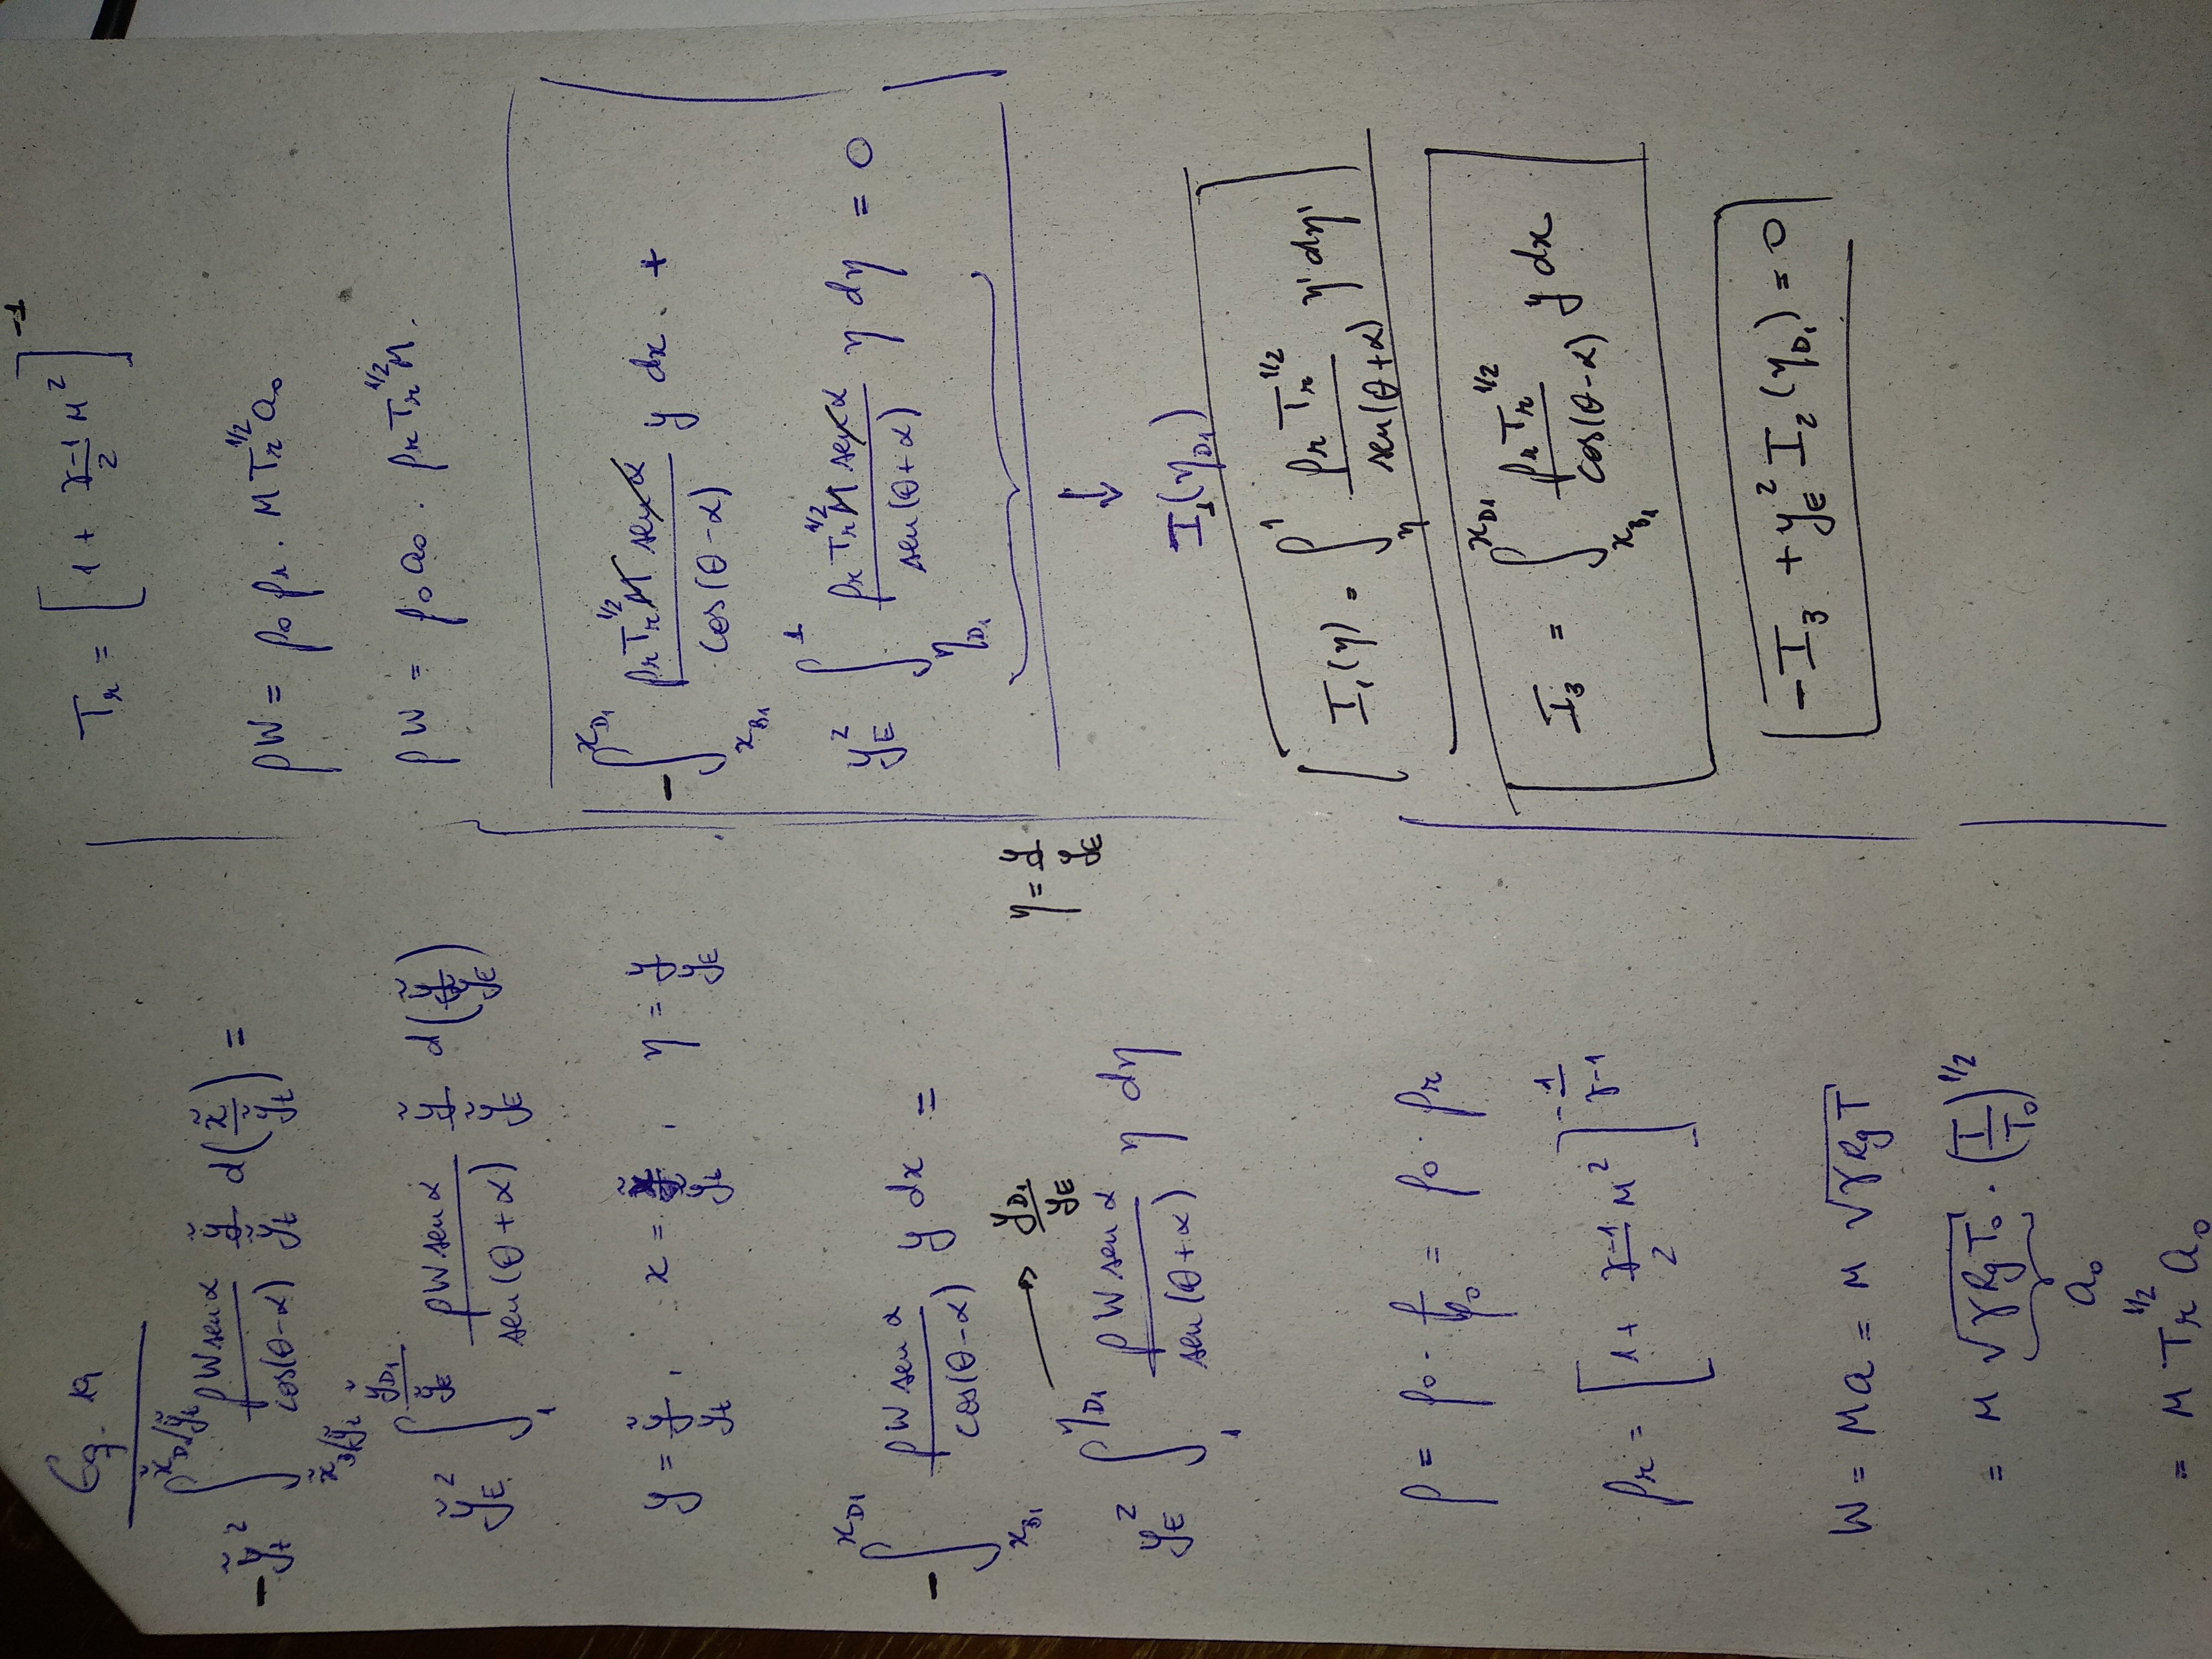
\includegraphics[width=0.95\textwidth, angle=-90]{./fig/eq19}
	\caption{Equação 19 do artigo do Rao na forma adimensional}
	\label{fig:Rao19}
\end{figure}
\begin{figure}[!ht]
	\centering
	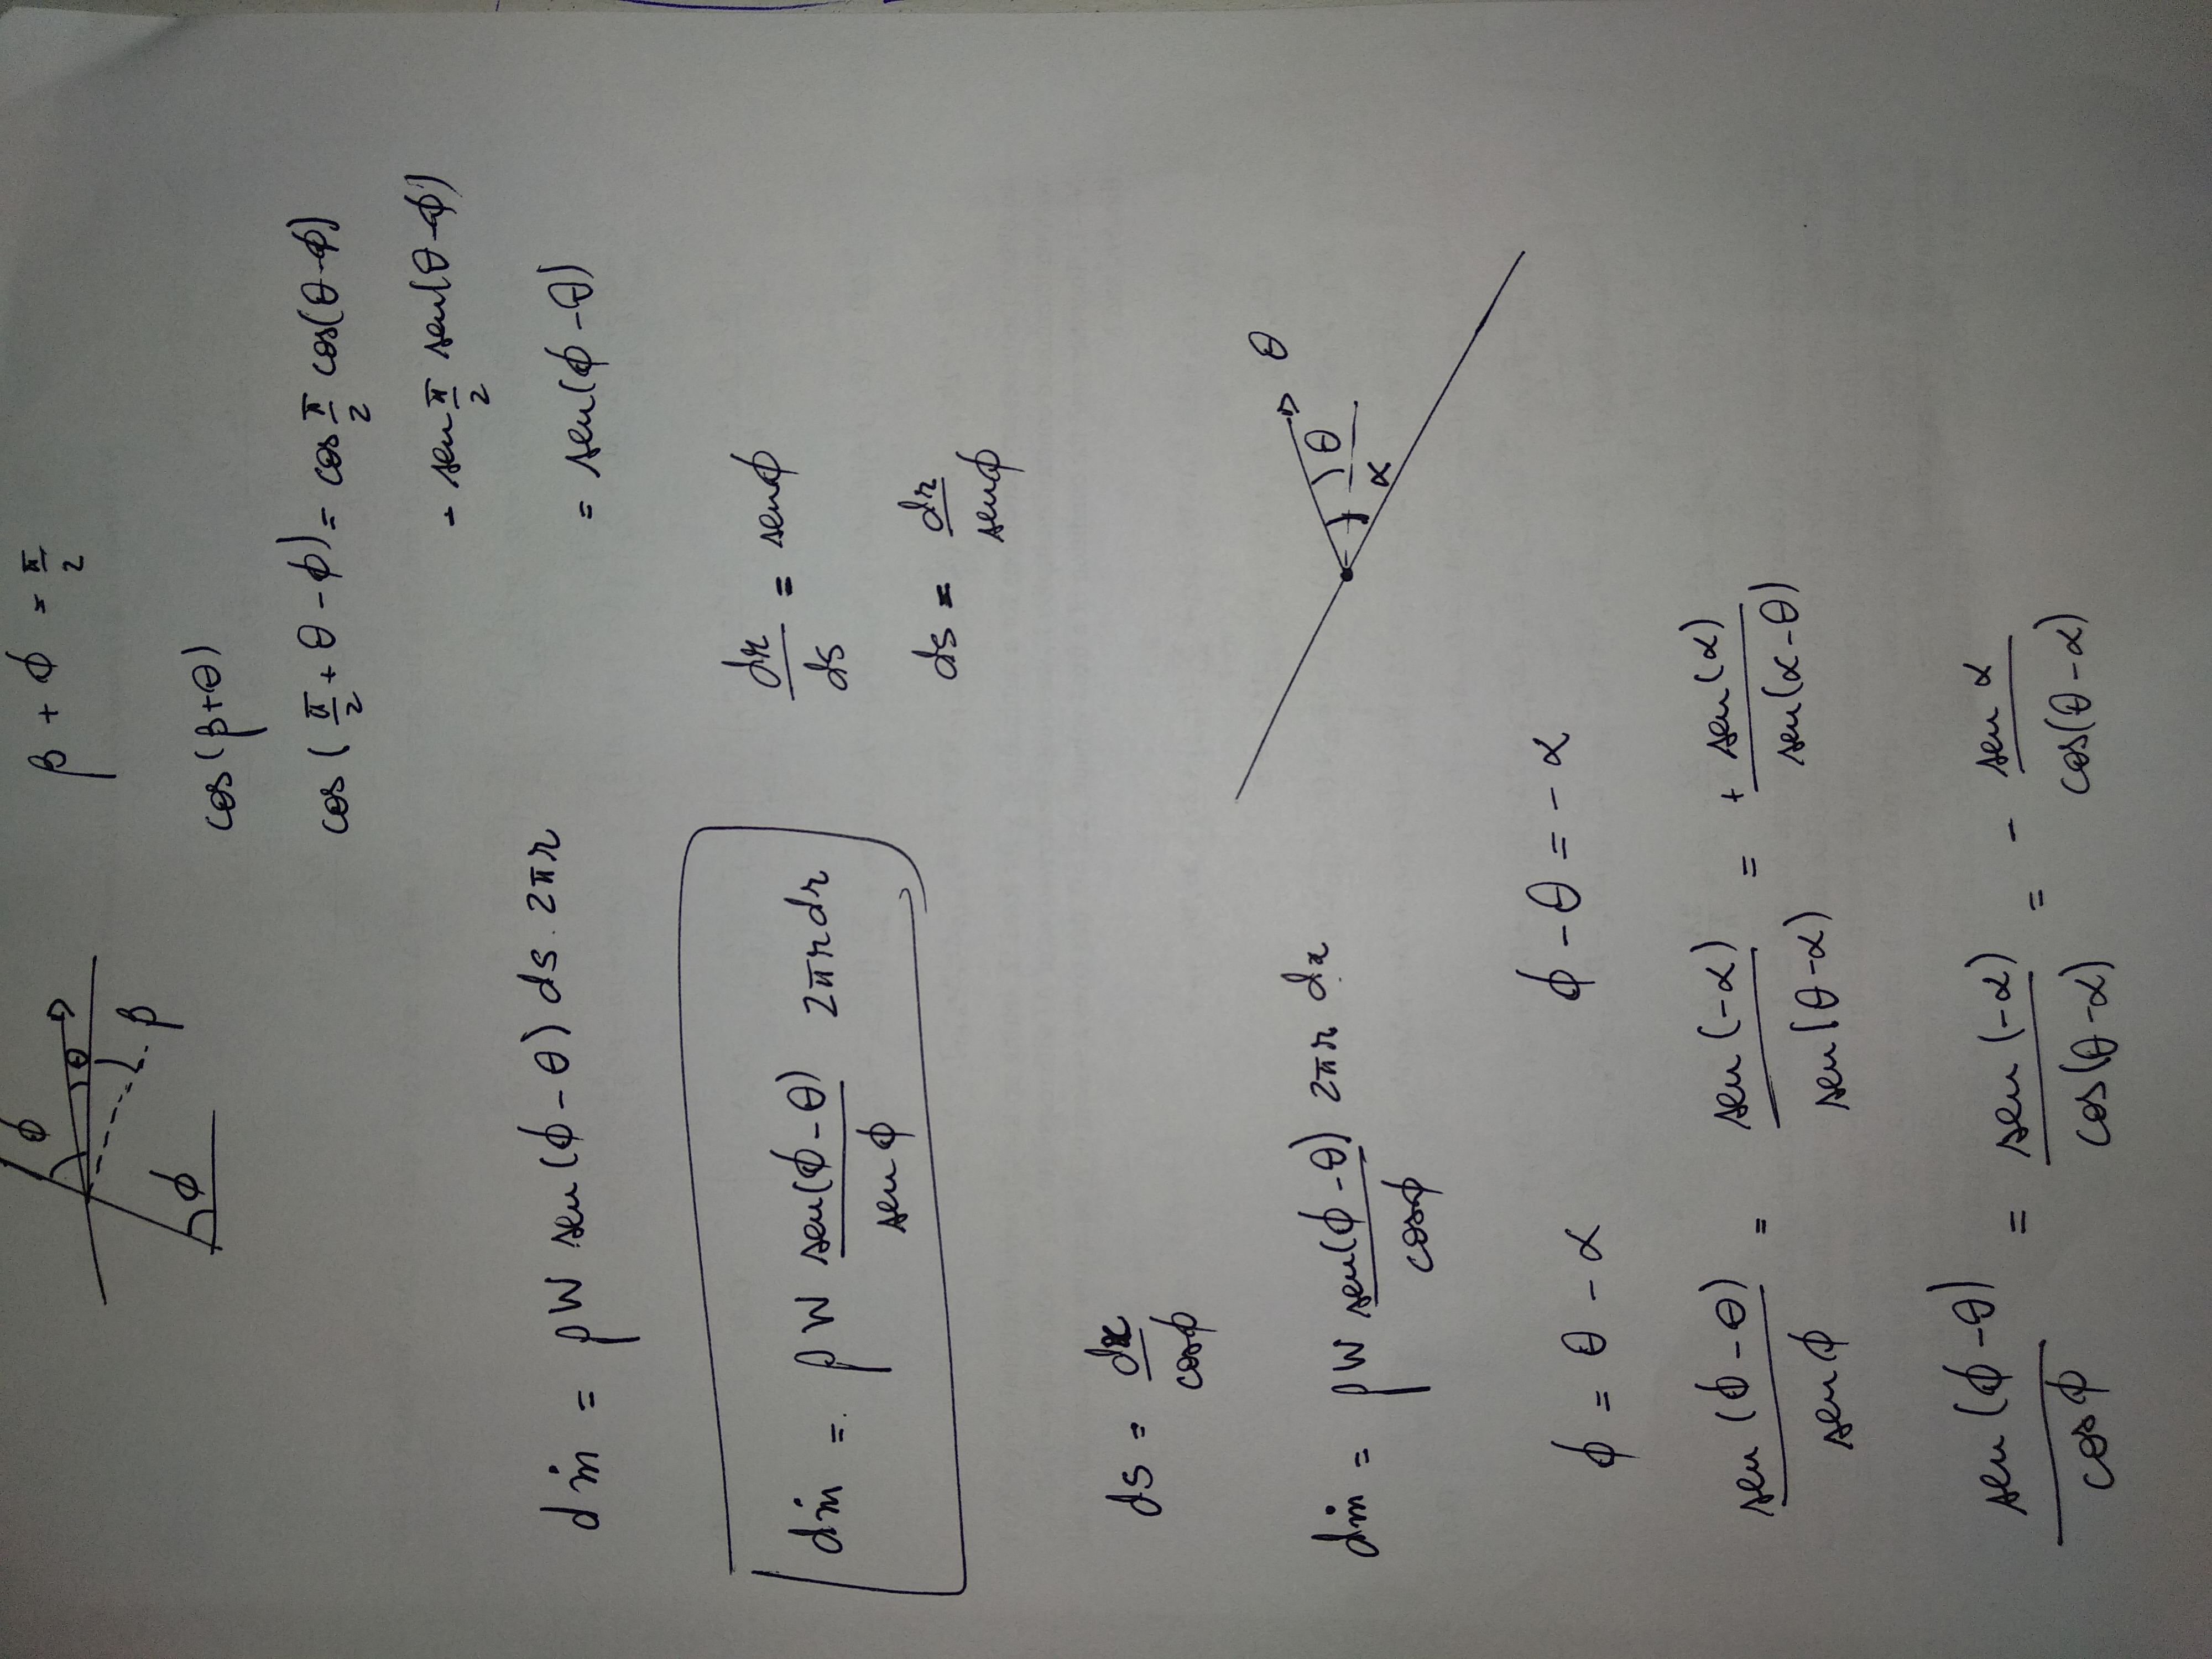
\includegraphics[width=0.95\textwidth, angle=-90]{./fig/eq19a}
	\caption{Equação 19 do artigo do Rao na forma adimensional}
	\label{fig:Rao19a}
\end{figure}
\begin{figure}[!ht]
	\centering
	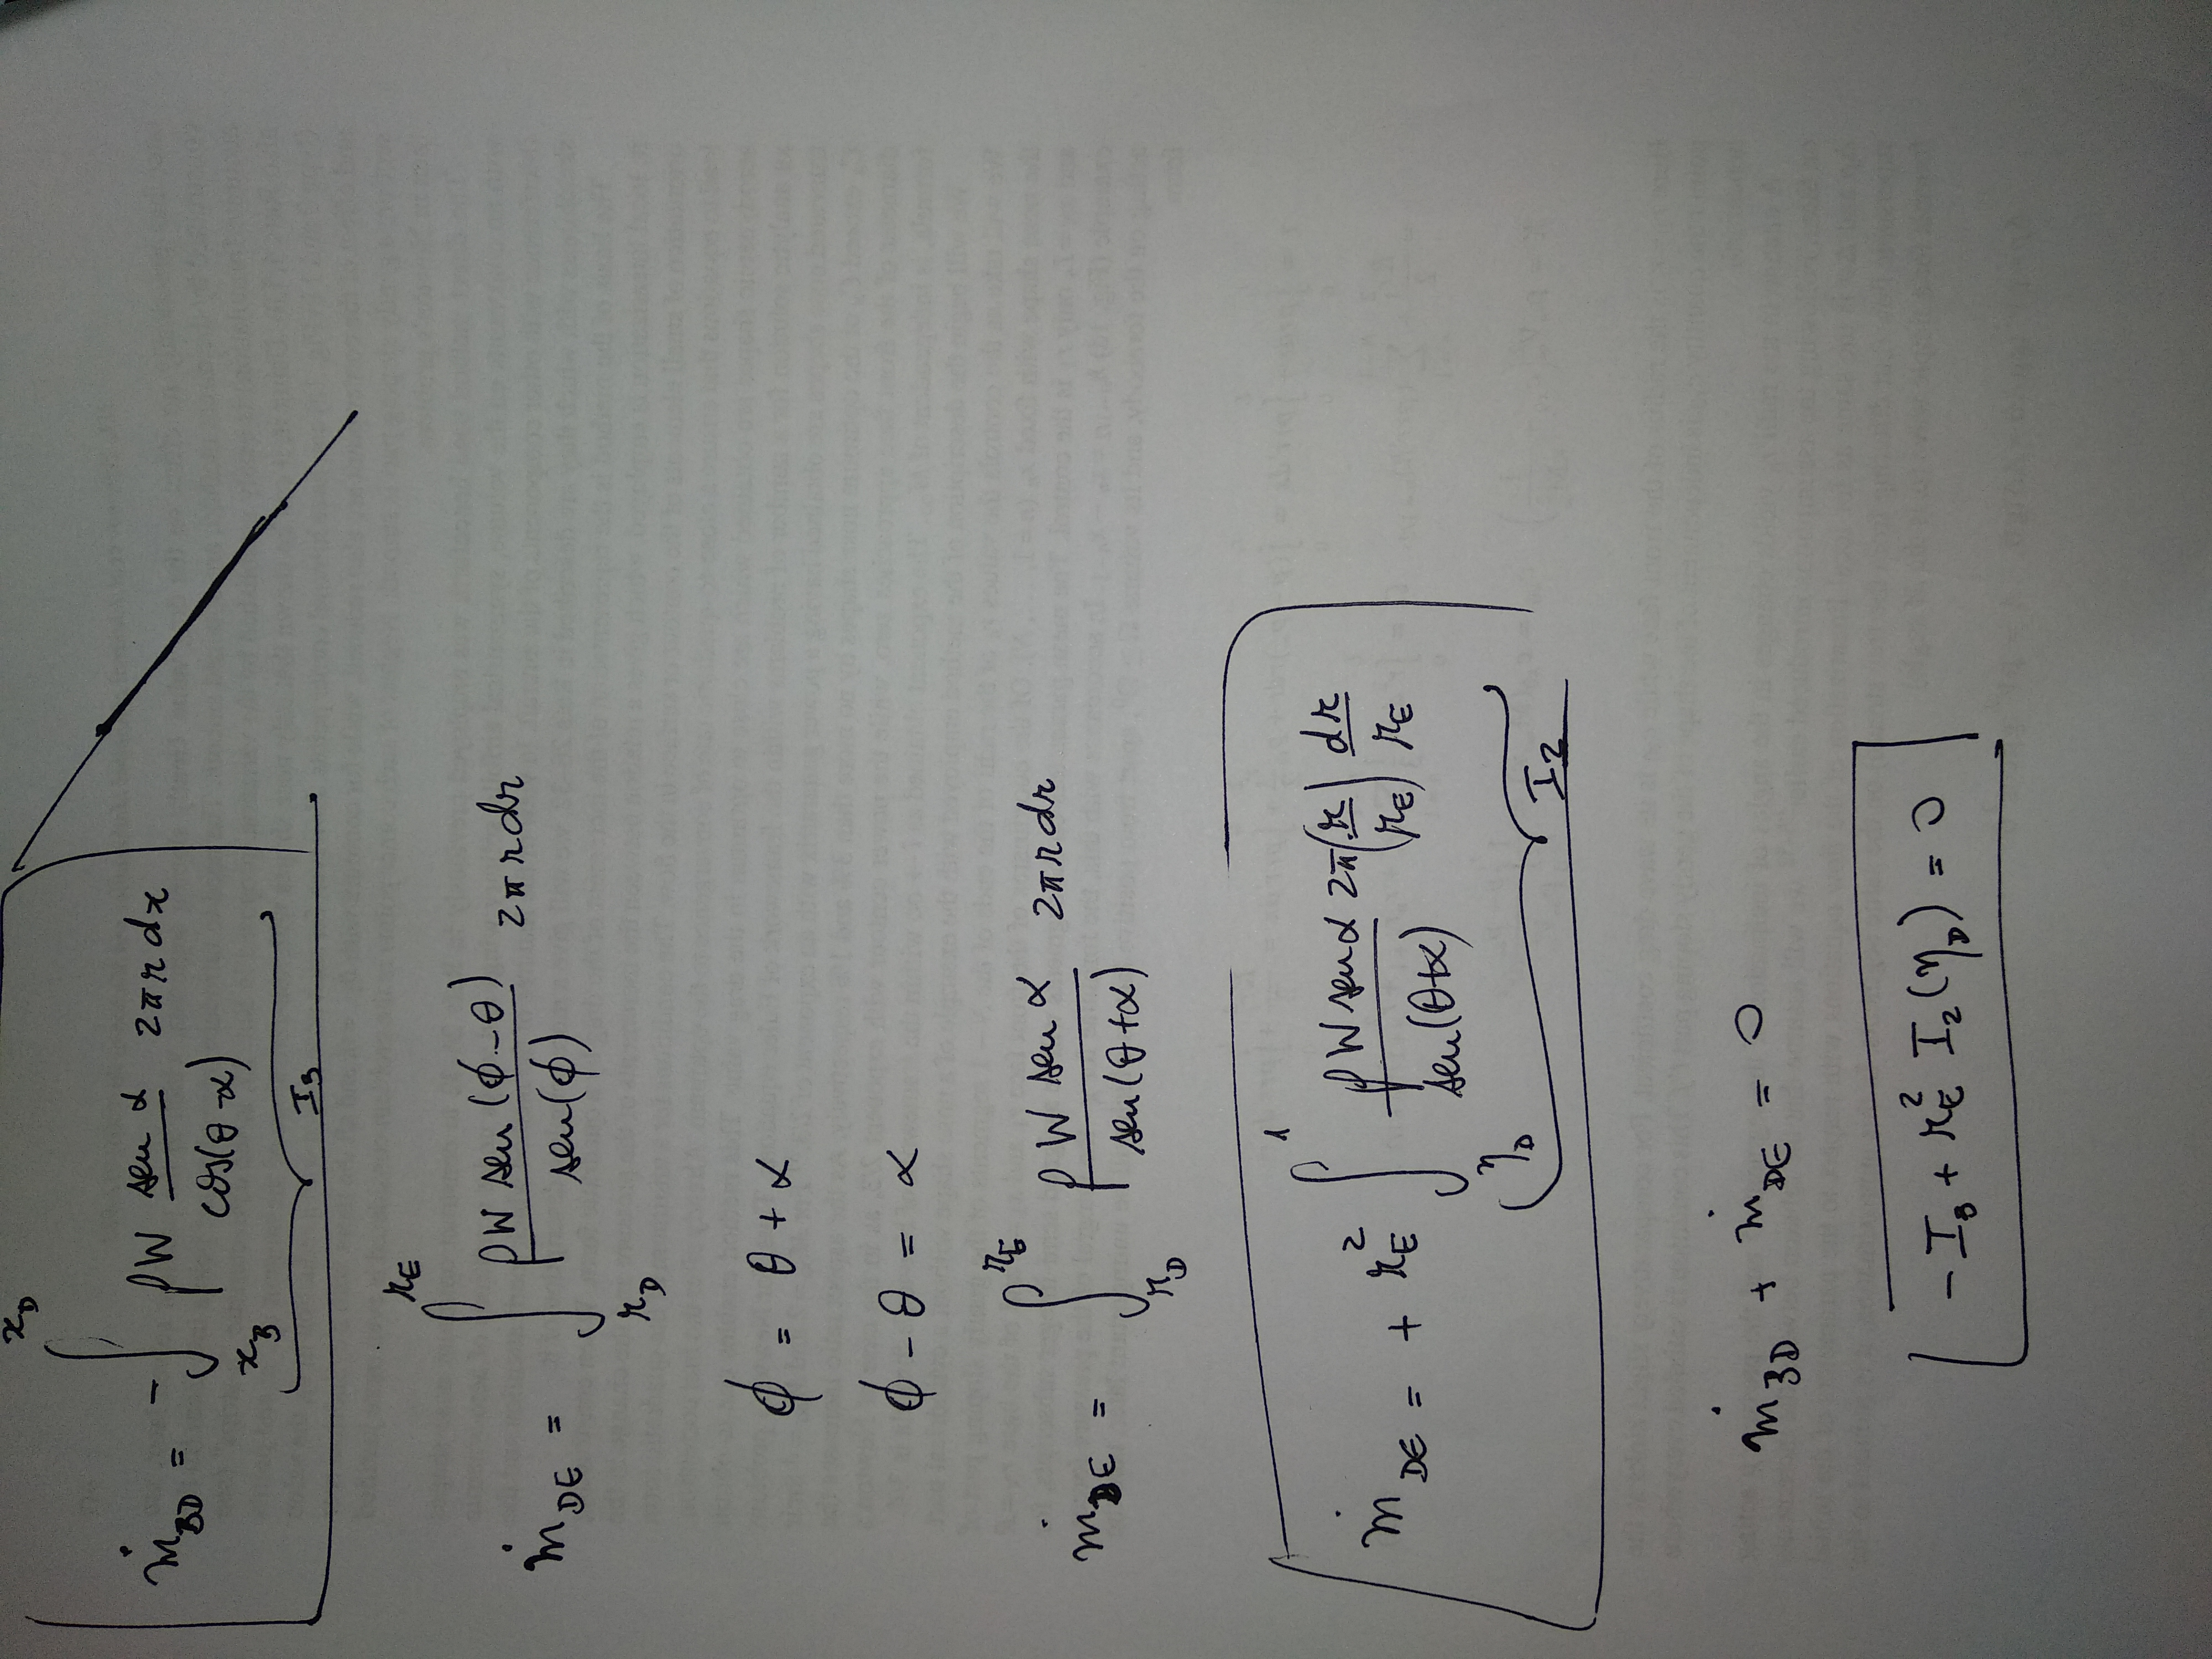
\includegraphics[width=0.95\textwidth, angle=-90]{./fig/eq19b}
	\caption{Equação 19 do artigo do Rao na forma adimensional}
	\label{fig:Rao19b}
\end{figure}
\newpage

\section{Coef. de empuxo - Eq.~(2) do artigo do Rao na forma adimensional}

\begin{figure}[!ht]
	\centering
	\includegraphics[width=0.90\textwidth]{./fig/CT1}
	\caption{Coeficiente de empuxo - parte 1}
	\label{fig:CT1}
\end{figure}

\begin{figure}[!ht]
	\centering
	\includegraphics[width=0.95\textwidth]{./fig/CT2}
	\caption{Coeficiente de empuxo - parte 2}
	\label{fig:CT2}
\end{figure}

\begin{figure}[!ht]
	\centering
	\includegraphics[width=0.95\textwidth]{./fig/CT3}
	\caption{Coeficiente de empuxo - parte 3}
	\label{fig:CT3}
\end{figure}

\end{document}
